\documentclass[kpfonts]{patmorin}
\usepackage{pat}
\usepackage{paralist}
\usepackage{dsfont}  % for \mathds{A}
\usepackage[utf8]{inputenc}

\usepackage{graphicx}

\newcommand{\snote}[1]{\fcolorbox{red}{yellow}{#1}}
\newcommand{\pnote}[1]{\ \newline\noindent\fcolorbox{red}{yellow}{\begin{minipage}{\textwidth}#1\end{minipage}}}
\setlength{\parskip}{1ex}

\DeclareMathOperator{\A}{\mathds{A}}
\DeclareMathOperator{\sn}{sn}
\DeclareMathOperator{\qn}{qn}

\renewcommand{\SS}{\mathcal{S}}


\newcommand{\aref}[1]{(X\ref{a:#1})}
\newcommand{\alabel}[1]{\label{a:#1}}

\title{\MakeUppercase{Optimal Adjacency-Labelling Schemes for Planar Graphs}}
\author{Barbados Folks}

\begin{document}
\begin{titlepage}
\maketitle

\begin{abstract}
  We describe an adjacency labelling-scheme for $n$-vertex planar graphs that assings each vertex a label of length $\log_2 n+o(\log n)$.  
\end{abstract}
\end{titlepage}
\pagenumbering{roman}
\tableofcontents

\newpage

\setcounter{page}{0}
\pagenumbering{arabic}
\section{Introduction}

In this paper, which is about binary encodings, $\log x:=\log_2 x$ denotes the binary logarithm of $x$.  We show that there exists an adjacency labelling scheme for planar graphs where each vertex of an $n$-vertex planar graph is assigned a $(\log n+o(\log n))$-bit label.  This is optimal up to the lower-order term.


\subsection{Proof Overview}

Like Bonamy \etal\ \cite{bonamy.gavoille.ea:shorter}.  Our starting point is a recent result that characterizes planar graphs in terms of the strong product of two simpler graphs.  The \emph{strong product} $A\boxtimes B$ of two graphs $A$ and $B$ is the graph whose vertex set is the Cartesian product $V(A\boxtimes B):=V(A)\times V(B)$ and in which two vertices $v_1:=(x_1,y_1)$ and $v_2:=(x_2,y_2)$ are adjacent if and only if:
\begin{enumerate}
  \item  $v_1\neq v_2$; and
  \item $x_1=x_2$ or $x_1x_2\in E(A)$; and
  \item $y_1=y_2$ or $y_1y_2\in E(B)$.
\end{enumerate}

\begin{thm}[Dujmović \etal \cite{dujmovic.joret.ea:planar}]
  Every planar graph $G$ is the subgraph of a strong product $G^+:=H\boxtimes P$ where $H$ is a graph of treewidth at most 8 and $P$ is a path.
\end{thm}

For graph products like $G^+$, there is a natural labelling scheme: Computer a labelling scheme $\alpha:V(H)\to\{0,1\}^*$ for $H$ and a labelling scheme $\beta:V(P)\to\{0,1\}^*$ for $P$ and assign each vertex $v:=(x,y)\in V(G^*)$ the label $\mu(v):=\alpha(x),\beta(y)$.  Given two labels $\ell_1=\alpha(x_1),\beta(y_1)$ and $\ell_2=\alpha(x_2),\beta(y_2)$ for vertices $v_1=(x_1,y_1)$ and $v_2=(x_2,y_2)$ adjacency testing is done using the following formula whose three clauses follow from definition of strong product:
\[
    L(\ell_1,\ell_2):= (\ell_1\neq \ell_2) \wedge \A(\alpha(x_1),\alpha(x_2)) \wedge \A(\beta(y_1),\beta(y_2)) \enspace .
\]

\ldots



\section{Preliminaries}

For a graph $G$, we use $V(G)$ and $E(G)$ to denote the vertex and edge sets of $G$.  We use $|G|$ as a shorthand for $|V(G)|$. For a vertex $v\in V(G)$, let $N_G(v):=\{w\in V(G): vw\in E(G)\}$ and $B_G(v):=N_G(v)\cup\{v\}$ denote the open neighbourhood and closed neighbourhood of $v$ in $G$, respectively.

For a string $s=s_1,\ldots,s_k$, we use $|s|:=k$ to denote the length of $s$. A string $s_1,\ldots,s_k$ is \emph{prefix} of a string $t_1,\ldots,t_\ell$ if $k\le \ell$ and $s_1,\ldots,s_k=t_1,\ldots,t_k$.  A \emph{prefix-free code} $c:X\to\{0,1\}^*$ is a one-to-one function in which $c(x)$ is not a prefix of $c(y)$ for any two distinct $x,y\in X$.  Let $\N$ denote the set of non-negative integers.  The following is an old result of Elias:

\begin{lem}[Elias \cite{elias:universal}]\lemlabel{elias}
    There exist a prefix-free code $\gamma:\N\to\{0,1\}^*$ such that, for each $i\in\N$, $|\gamma(i)|\le 2\lfloor\log(i+1)\rfloor + 1\in O(\log(i+1))$.
\end{lem}

A \emph{binary tree} $T$ is a rooted binary tree in which each node except the root is either the \emph{left} or \emph{right} child of its parent and each node has at most one left and at most one right child.  For any node $v$ in $T$, $P_T(v)$ denotes the path from the root of $T$ to $v$.  The \emph{length} of a path $P$ is the number of edges in $P$.  The \emph{depth}, $d_T(v)$ of $v$ is the length of $P_T(v)$.  The \emph{height} of $T$ is $h(T):=\max_{v\in V(T)} d_T(v)$.  A \emph{perfectly balanced} binary tree is any binary tree $T$ with $h(T)=\lfloor\log|T|\rfloor$.

A node $a\in V(T)$ is an \emph{ancestor} of $v\in V(T)$ if the path in $T$ from the root of $T$ to $v$ includes $a$.  (Note that $v$ is an ancestor of itself.) For a node subset $X\subseteq V(T)$, the \emph{lowest common ancestor} of $X$ is the maximum-depth node $a\in V(T)$ such that $a$ is an ancestor of $v$ for each $v\in X$.

Let $v_0,\ldots,v_{r}$ be a path from the root $v_0$ of $T$ to some node $v_r$ (possibly $r=0$).  Then the \emph{signature} of $v_r$ in $T$, denoted $\sigma_T(v_r)$ is a binary string $b_1,\ldots,b_r$ where $b_i=0$ if and only if $v_{i}$ is the left child of $v_{i-1}$.  (Note that the signature of the root $v_0$ of $T$ is the empty string,  $\sigma_T(v_0)=\varepsilon$.)

A \emph{binary search tree (BST)} $T$ is a binary tree  whose node set $V(T)\subset\R$ consists of real numbers and that has the \emph{BST property}:  For each node $x$, $z<x$ for each node $z$ in $x$'s left subtrees and $z>x$ for each node $z$ in $x$'s right subtree. The following observation allows us to replace (possibly large) numbers with (potentially shorter) binary strings:

\begin{obs}\obslabel{lexicographic}
  If $T$ is a binary search tree then, for any $x,y\in V(T)$, $x<y$ if and only if $\sigma_T(x)$ is lexicographically less than $\sigma_T(y)$.
\end{obs}

Let $\R^+$ denote the set of positive real numbers. The following is an easy and often-used result about biased binary search trees:

\begin{lem}\lemlabel{biased-bst}
  For any function $w:\{1,\ldots,n\}\to\R^+$, there exists a binary search tree $T$ containing $\{1,\ldots,n\}$ such that, for each $i\in\{1,\ldots,n\}$, $d_T(i)\le\log(W/w(i))$, where $W:=\sum_{i=1}^n w(i)$.
\end{lem}

To construct the tree in \lemref{biased-bst}, choose the root of $T$ to be the unique node $x\in\{1,\ldots,n\}$ such that $\sum_{z=1}^{x-1} w(i)\le W/2$ and $\sum_{z=x+1}^{n} w(i)< W/2$.  Then recurse on $\{1,\ldots,x-1\}$ and $\{x+1,\ldots,n\}$ to obtain the left and right subtrees, respectively.

The following fact about binary search trees is useful, for example, in the deletion algorithms for several types of balanced binary search trees \cite[Section~6.2.3]{morin:open}:

\begin{lem}\lemlabel{predecessor-encoding}
  Let $T$ be a binary search tree and let $x,y\in V(T)$ be such that $x<y$ and there is no node $z\in V(T)$ such that $x<z<y$ (i.e., $x$ and $y$ are consecutive in the sorted order of $V(T)$).  Then
  \begin{enumerate}
    \item (if $x$ has no left child) $\sigma_T(y)$ is obtained from $\sigma_T(x)$ by removing all trailing 0's and the last 1; or
    \item (if $x$ has a left child) $\sigma_T(y)$ is obtained from $\sigma_T(x)$ by appending a 0 followed by $s:=d_T(y)-d_T(x)-1$ 1's.
  \end{enumerate}
\end{lem}

Putting some of the preceding results together we obtain the following useful coding result:

\begin{lem}\lemlabel{row-code}
  The exists a function $A:(\{0,1\}^*)^2\to\{-1,1,\perp\}$ such that, for any $h\in\N$, and any $w:\{1,\ldots,h\}\to\R^+$ there is a prefix-free code $\alpha:\{1,\ldots,h\}\to \{0,1\}^*$ such that 
  \begin{compactenum}
    \item for each $i\in\{1,\ldots,h\}$, $|\alpha(i)|=\log W -\log w(i) + O(\log\log h)$; and
    \item for each distinct $i,j\in\{1,\ldots,h\}$, 
    \[   A(\alpha(i),\alpha(j)) 
    = \begin{cases}
       1 & \text{if $j=i+1$} \\
       -1 & \text{if $j=i-1$} \\
       \perp & \text{otherwise}
      \end{cases}
      \]
    \end{compactenum}
\end{lem}


\begin{proof}
  Define $w':\{1,\ldots,h\}\to \R^+$ as $w'(i)=w(i)+W/h$ and let $W':=\sum_{i=1}^h w'(i)=2W$.
  Using \lemref{biased-bst}, construct a biased binary search tree $T$ on $\{1,\ldots,h\}$ using $w'$ so that 
  \[   
    d_T(i)\le\log (2W)-\log(w(i)+W/h) \le \log W-\log w(i)+1 \enspace .
  \]
  Also
  \[
  d_T(i)\le\log (2W)-\log(w(i)+W/h) \le \log W-\log (W/h)+1 \le \log h + 1\enspace .
  \]
  for each $i\in\{1,\ldots,h\}$.  The code $\alpha(i$) for $i$ consists of three parts.  The first part, $\gamma(|\sigma_T(i)|)$, encodes the length of the path from the root to $i$ in $T$. The second part $\sigma_T(i)$ encodes the left/right turns along this path.  
  
  The third part $\delta(i)$ of $\alpha(i)$ is the encoding implicit in \lemref{predecessor-encoding}.  That is $\delta(i)$ consists of
  a single bit indicating whether $i$ has a left-child in $T$ and, in case $i$ does have a left-child, an Elias encoding of the value $s=d_T(i-i)-d_T(i)-1$.  More precisely, $\delta(i)=0$ or $\delta(i)=1,\gamma(s)$.  The length of $\delta(i)$ is at most $1+O(\log(s+1))=O(\log\log h)$.

  The function $A$ is now given by a simple algorithm: Given $\alpha(i)$ and $\alpha(j)$ we extract and lexicographically compare $\sigma_T(i)$ and $\sigma_T(j)$.  Assume, for now that $\sigma_T(i)$ is lexicographically less than $\sigma_T(j)$ so that, by \obsref{lexicographic}, $i < j$.  Now using $\sigma_T(j)$ and $\delta(j)$, compute $\sigma_T(j-1)$.  If $\sigma_T(j-1)=\sigma_T(i)$ then output $1$, otherwise output $\perp$.
  In the case where $\sigma_T(i)$ is lexicographically greater than $\sigma_T(j)$ we proceed in the same manner, but reversing the roles of $i$ and $j$ and outputting $-1$ in the case where $\sigma_T(i-1)=\sigma_T(j)$.
\end{proof}

\section{Subgraphs of $P\boxtimes P$}
\seclabel{pxp}

We begin with the special case where $G$ is an $n$-vertex subgraph of $P_1\boxtimes P_2$ where $P_1=1,\ldots,m$ and $P_2=1,\ldots,h$ are paths, so that each vertex of $G$ is a pair $(x,y)\in\{1,\ldots,m\}\times \{1,\ldots,h\}$. The graph $P_1\boxtimes P_2$ is an $m\times h$ grid-with diagonals.  

% \pnote{TODO: Annoyingly, I now have to reverse the roles of $x$ and $y$ so that, in $H\boxtimes P$, $x\in V(H)$ and $y\in V(P)$. }

\subsection{The Labels}

For each $y\in\{1,\ldots,h\}$, we let $L_y=\{x\in\{1,\ldots,m\}:(x,y)\in V(G)\}$.  The idea behind our approach is to have a sequence $T_1,\ldots,T_h$ of balanced binary search trees where, for each $y\in\{1,\ldots,h\}$,
\begin{enumerate}[(PR1)]
  \item $T_y$ contains (a superset of) $\bigcup_{b\in\{0,1\}} (L_{y+b}\cup \{x-1:x\in L_{y+b}\})$;
  \item The height $h(T_y)$ of $T_y$ is $\log |T_y| + o(\log n)$;
  \item $W:=\sum_{y=1}^h |T_y| = O(n)$;
  \item If $x\in V(T_y)\cap V(T_{y+1})$, then $\sigma_{T_{y+1}}(x)$ can be obtained from $\sigma_{T_{y}}(x)$ with an additional $o(\log n)$ bits that we denote by $\nu_x(y)$.  More precisely, there is a function $B:(\{0,1\}^*)^2\to\{0,1\}^*$ such that $B(\sigma_{T_{y}}(x), \nu_y(x))=\sigma_{T_{y+1}}(x)$
\end{enumerate}

Before describing the sequence of trees satisfying (PR1--4), we show how these can be used in a labelling scheme for $G$. 

Given $G$ and $T_{1},\ldots,T_h$ we use a \lemref{row-code} with the weight function $w(y):=|T_y|$ to construct a code $\alpha:\{1,\ldots,h\}\to\{0,1\}^*$ where
\[  
  |\alpha(y)| = \log W-\log|T_y| + O(\log\log h) = \log n - \log|T_y| + O(\log\log n)
\]
for each $y\in\{1,\ldots,h\}$.  Every vertex $z=(x,y)\in V(G)$ receives a label consisting of the following:  
\begin{enumerate}[(GC1)]
  \item $\alpha(y)$;
  \item $\gamma(|\sigma_{T_y}(x)|)$ and $\sigma_{T_y}(x)$;    
  \item $\delta_{T_y}(x)$;
  \item $\nu_y(x)$; and
  \item an array $a(v)$ of $8$ bits indicating whether each of the edges between $(x,y)$ and $(x\pm 1,y\pm 1)$ are present in $G$.  (Note that some of these 8 vertices may not even be present in $G$ in which case the resulting bit is set to 0 since the edge is not present in $G$.)
\end{enumerate}
The two major components of this label are $\alpha(y)$ (GC1) and $\sigma_{T_y}(x)$ (GC2) which, together have length $\log n + O(\log\log n)$.  The remaining components have size $O(|\nu_y(x)|+\log\log n)$.  

A large part of the remaining work involves describing $\nu_y(x)$ and, ultimately, showing that $|\nu_y(x)|\in O(\sqrt{\log n\log\log n})$. First, though, we show how (GC1)--(GC5) can be used for adjacency testing.

\subsection{Adjacency Testing}

Given the labels of $z_1=(x_1,y_1)$ and $z_2=(x_2,y_2)$ we can test if they are adjacent as follows: Using \lemref{row-code} with $\alpha(y_1)$ and $\alpha(y_2)$, determine which of the following applies:
\begin{enumerate}
  \item $|y_1-y_2|\ge 2$: In this case we immediately conclude that $z_1$ and $z_2$ are not adjacent since $y_1y_2\not\in E(P_1)$.  
  
  \item $y_1=y_2$: In this case, let $y:=y_1=y_2$, let $T:=T_y$ and lexicographically compare $\sigma_T(x_1)$ and $\sigma_T(x_2)$ to determine (without loss of generality) that $x_1<x_2$.  Using $\sigma_{T}(x_2)$ and $\delta_{T}(x_2)$, compute $\sigma{T}(x_2-1)$.  If $\sigma_T(x_2-1)\neq \sigma_T(x_1)$ then immediately conclude that $z_1$ and $z_2$ are not adjacent, since $x_1x_2\not\in E(P_2)$.  Otherwise, we know that $x_1=x_2-1$ and $y_1=y_2$ so use the relevant bit of $a(z_1)$ (or $a(z_2)$) to determine if $z_1$ and $z_2$ are adjacent in $G$.
  
  \item $y_1=y_2-1$: In this case, use $\sigma_{T_{y_1}}(x_1)$ and $\nu_{y_1}(x_1)$ to compute $\sigma_{T_{y_2}}(x_1)$.  Now let $y:=y_2$, let $T:=T_{y}$, and proceed as in the previous case (but consulting a different bit of $a(z_1)$ in the last step.)
  
  \item $y_2=y_1-1$: In this case, use $\sigma_{T_{y_2}}(x_2)$ and $\nu_{y_2}(x_2)$ to compute $\sigma_{T_{y_1}}(x_2)$.  Now let $y:=y_1$, $T:=T_{y}$, and proceed as in the previous case (but consulting a different bit of $a(z_1)$ in the last step.)
\end{enumerate}

Thus, all that remains is to find a sequence of binary search trees $T_1,\ldots,T_h$ with properties (PR1)--(PR4). This is a data structuring problem and we use a combination of existing and new techniques from data structures to solve it.

\subsection{Fractional Cascading}

Ultimately, we want to reach a point where, for each $y\in\{1,\ldots,h-1\}$ and each $x\in V(T_y)\cap V(T_{y+1})$, the difference between $\sigma_{T_y}(x)$ and $\sigma_{T_{y+1}}(x)$ has a description $\nu_x(y)$ of length $o(\log n)$.  In order for this to be possible, we require that $V(T_y)$ not be wildly different from $V(T_{y+1})$.  In the world of data structures, this is achieved by the technique of \emph{fractional cascading} \cite{chazelle.guibas:fractional1, chazelle.guibas:fractional2, vaishnavi.wood:rectilinear}.

For non-empty sets $X,Y\subset \R$ and an integer $a$, we say that $X$ \emph{$a$-chunks} $Y$ if, for any $a+1$-element subset $S\subseteq Y$, there exists $x\in X$, such that $\min(S)\le x\le \max(S)$. Observe that, if $X$ $a$-chunks $Y$, then $|Y|\le a(|X|+1)\le 2a|X|$.

For each $y\in\{1,\ldots,h\}$, let $L^-_y:=L_y\cup \{x-1:x\in L_y\}$ and observe that $|L^-_y|\le 2|L_y|$, so $\sum_{x=1}^h|L^-_y| \le 2n$.  The following lemma is a form of fractional cascading.  A proof of (a much more general version of) this lemma is implicit in the iterated search structure of Chazelle and Guibas \cite{chazelle.guibas:fractional1}.   \snote{Put a self-contained proof in the appendix?}

\begin{lem}\lemlabel{fractional}
  There exists universal constants $a,b\ge 1$ and sets $V_1,\ldots,V_m$ such that
  \begin{compactenum}
    \item for each $y\in\{1,\ldots,m\}$, $V_y\supseteq L^-_y$;
    \item for each $y\in\{1,\ldots,m-1\}$, $V_y$ $a$-chunks $V_{y+1}$ and $V_{y+1}$ $a$-chunks $V_y$; and
    \item $\sum_{y=1}^m |V_y|\le bn$.
  \end{compactenum}
\end{lem}

Condition~2 in \lemref{fractional} has the following interpretation:  If we sort $V_y\cup V_{y+1}$, then we never see more than $a$ consecutive elements that only belong only to $V_y$ nor do we ever see more than $a$ consecutive elements that belong only to $V_{y+1}$.

We will use \lemref{fractional} to creating the sequence of binary search trees $T_1,\ldots,T_h$ where $V(T_y):=V_y$ for each $y\in\{1,\ldots,m\}$.  Condition~2 in \lemref{fractional} is what will ultimately make it possible to have $T_y$ and $T_{y+1}$ sufficiently similar so that, for any $x\in V_y\cap V_{y+1}$, there will be an $o(\log n)$-bit description $\nu_y(x)$ of how to modify $\sigma_{T_y}(x)$ in order to obtain $\sigma_{T_{y+1}}(x)$.  To begin with, we describe the three operations bulk deletions, bulk insertions, and rebalancing that transform $T_y$ into $T_{y+1}$.

\subsection{Bulk Deletions}

\begin{lem}\lemlabel{deletion-prefix}
  For any binary search tree $T$ and any $D\subseteq V(T)$, there exists a binary search tree $T'$ with $V(T')=V(T)\setminus D$ such that, for every $x\in V(T')$, $\sigma_{T'}(x)$ is a prefix of $\sigma_{T}(x)$.
\end{lem}

\begin{proof}
  It suffices to prove this for a singleton set $D$ containing one element $z$ since, for larger $D$ we can remove the values from $T$ one at a time.  The correctness of this follows from the transitivity of the ``is a prefix of'' relation on strings.
  
  The proof is by induction on $|T|$. If $|T|=1$, then the claim is vacuous since $V(T')=\emptyset$.  Therefore assume $|T|\ge 2$.  If $z$ is leaf in $T$, then use $T'=T-\{z\}$ and the result is trivial: $\sigma_{T'}(y)=\sigma_T(y)$ for every $y\in V(T')$.  
  
  Otherwise, $z$ has at least one child.  Without loss of generality, assume $z$ has a non-empty left subtree $T_l$.  Then the largest node $z'$ in $V(T_l)$ is the largest value in $V(T)$ that is less than $z$. Inductively remove $z'$ from $T_l$ to obtain $T_l'$ and make this the left child of $z$.  Now replace $z$ with $z'$ to obtain $T'$.  
  
  That $T'$ is indeed a binary search tree is straightforward to verify.  All that remains is to prove that $\sigma_{T'}(x)$ is a prefix of $\sigma_T(x)$ for every $x\in V(T')$. There are three cases:
  \begin{enumerate}
    \item $x=z'$: Since $z$ is an ancestor of $z'$ in $T$, $\sigma_{T'}(x)=\sigma_T(z)$ is a prefix of $\sigma_T(x)=\sigma_T(z')$.  
    
    \item $x\in V(T)\setminus\{z\}\setminus V(T_l)$: In this case $\sigma_T(x)=\sigma_{T'}(x)$.  
    
    \item $x\in V(T_l')$: In this case, $\sigma_{T'}(x)=\sigma_{T}(z),0,\sigma_{T_l'}(x)$ and $\sigma_T(x)=\sigma_{T}(z),0,\sigma_{T_l}(x)$.  By induction, $\sigma_{T_l'}(x)$ is a prefix of $\sigma_{T_l}(x)$, so $\sigma_{T'}(x)$ is a prefix of $\sigma_T(x)$. \qedhere
  \end{enumerate}
\end{proof}

\lemref{deletion-prefix} is useful because it means that, for any particular node of $x$ of $T_y$, the net effect of all the deletions performed when moving from $T_y$ to $T_{y+1}$ on $\sigma_{T_y}(x)$ can be encoded by a single integer in the range $\{0,\ldots,h(T_y\}$.  Using \lemref{elias}, this requires only $O(\log h(T_y))$ bits.  If $T$ is at-all balanced, this is only $O(\log\log n)$ bits.

\subsection{Bulk Insertions}

\begin{lem}\lemlabel{chunked-addition}
  For any binary search tree $T$ and any set $I\subset\R\setminus V(T)$ such that $V(T)$ $a$-chunks $I$, there exists a binary search tree $T'$ with $V(T')=V(T)\cup I$ that is a supergraph of $T$ and such that $h(T')\le h(T)+1+\log a$.
\end{lem}

\begin{proof}
  Search for each element $x\in I$ in $T$ until the search path falls out of $T$.  This would be the natural place to add $x$ as a leaf to $T$.  This partitions $I$ into $r:=|T|+1$ sets $I_1,\ldots,I_r$ and, since $V(T)$ $a$-chunks $I$, each $I_i$ has size at most $a$.  For each $I_i$ construct a binary search tree $T_i$ of height at most $\log a$ and attach this to the appropriate location in $T$ to obtain $T'$.
\end{proof}

\lemref{chunked-addition} is useful because the set of values $I:=V_{y+1}\setminus V_y$ that are present in $T_{y+1}$ but not in $T_y$ are $a$-chunked by $V_y$. Therefore, we can perform all the insertions required to move from $T_y$ to $T_{y+1}$ in such a way that $\sigma_{T_y}(x)=\sigma_{T_{y+1}}(x)$ for every $x\in V_y\cap V_{y+1}$ and $h(T_{y+1})\le h(T_y)+1+\log a$.  

\subsection{Tree Splitting}

\lemref{deletion-prefix} and \lemref{chunked-addition} help control the structure of the trees $T_1,\ldots,T_h$.  However, by themselves, they are not enough to ensure that $h(T_y)=\log|T_y|+o(\log n)$, even if $T_1$ is perfectly balanced.  Indeed, \lemref{deletion-prefix} does not ensure that the height of $T$ decreases even after many deletions.  Similarly, \lemref{chunked-addition} allows the height of $T$ to increase by $1+\log a$ even in the case where only $a$ additional elements are inserted.  

In this section, we introduce what (to our knowledge) is a novel form of rebalancing that ensures that $h(T_y)=\log|T_y|+o(\log n)$.  Standard forms of rebalancing, including height-balancing, weight-balancing, and partial rebuilding seem not to be applicable in our setting because we have unusual requirements.  In particular, the requirement $h(T_y)=\log|T_y|+o(\log n)$ is quite stringent. Most standard binary search trees guarantee only $h(T)\le c\log |T|$ for some some constant $c>1$.  Even more exotic is that the updates come in linear-sized batches, where batch $y$ consists of the deletions $D_y:=V_y\setminus V_{y+1}$ and the insertions $I_y:=V_{y+1}\setminus V_y$, and we require that there exists a simple relationship between $\sigma_{T_y}(x)$ and $\sigma_{T_{y+1}}(x)$ for each $x\in V_y\cap V_{y+1}$.     

We begin with the following simple lemma:

\begin{lem}\lemlabel{split}
  Let $T$ be a binary search tree and let $x$ be any node of $T$.  Then there exists a binary search tree $T'$ with $h(T')\le h(T)+1$, $V(T')=V(T)$ whose root is $x$ and such that, for each node $z\in V(T')$, $\sigma_{T'}(z)$ is obtained by replacing a prefix of $\sigma_{T}(z)$ with a binary string from the set $\{\varepsilon\}\cup \{01^r:r\in\{0,\ldots,h(T)\}\cup \{10^r:r\in\{0,\ldots,h(T)\}$.  
\end{lem}

\begin{proof}
Proof by (crappy) illustration:
  \begin{center}
    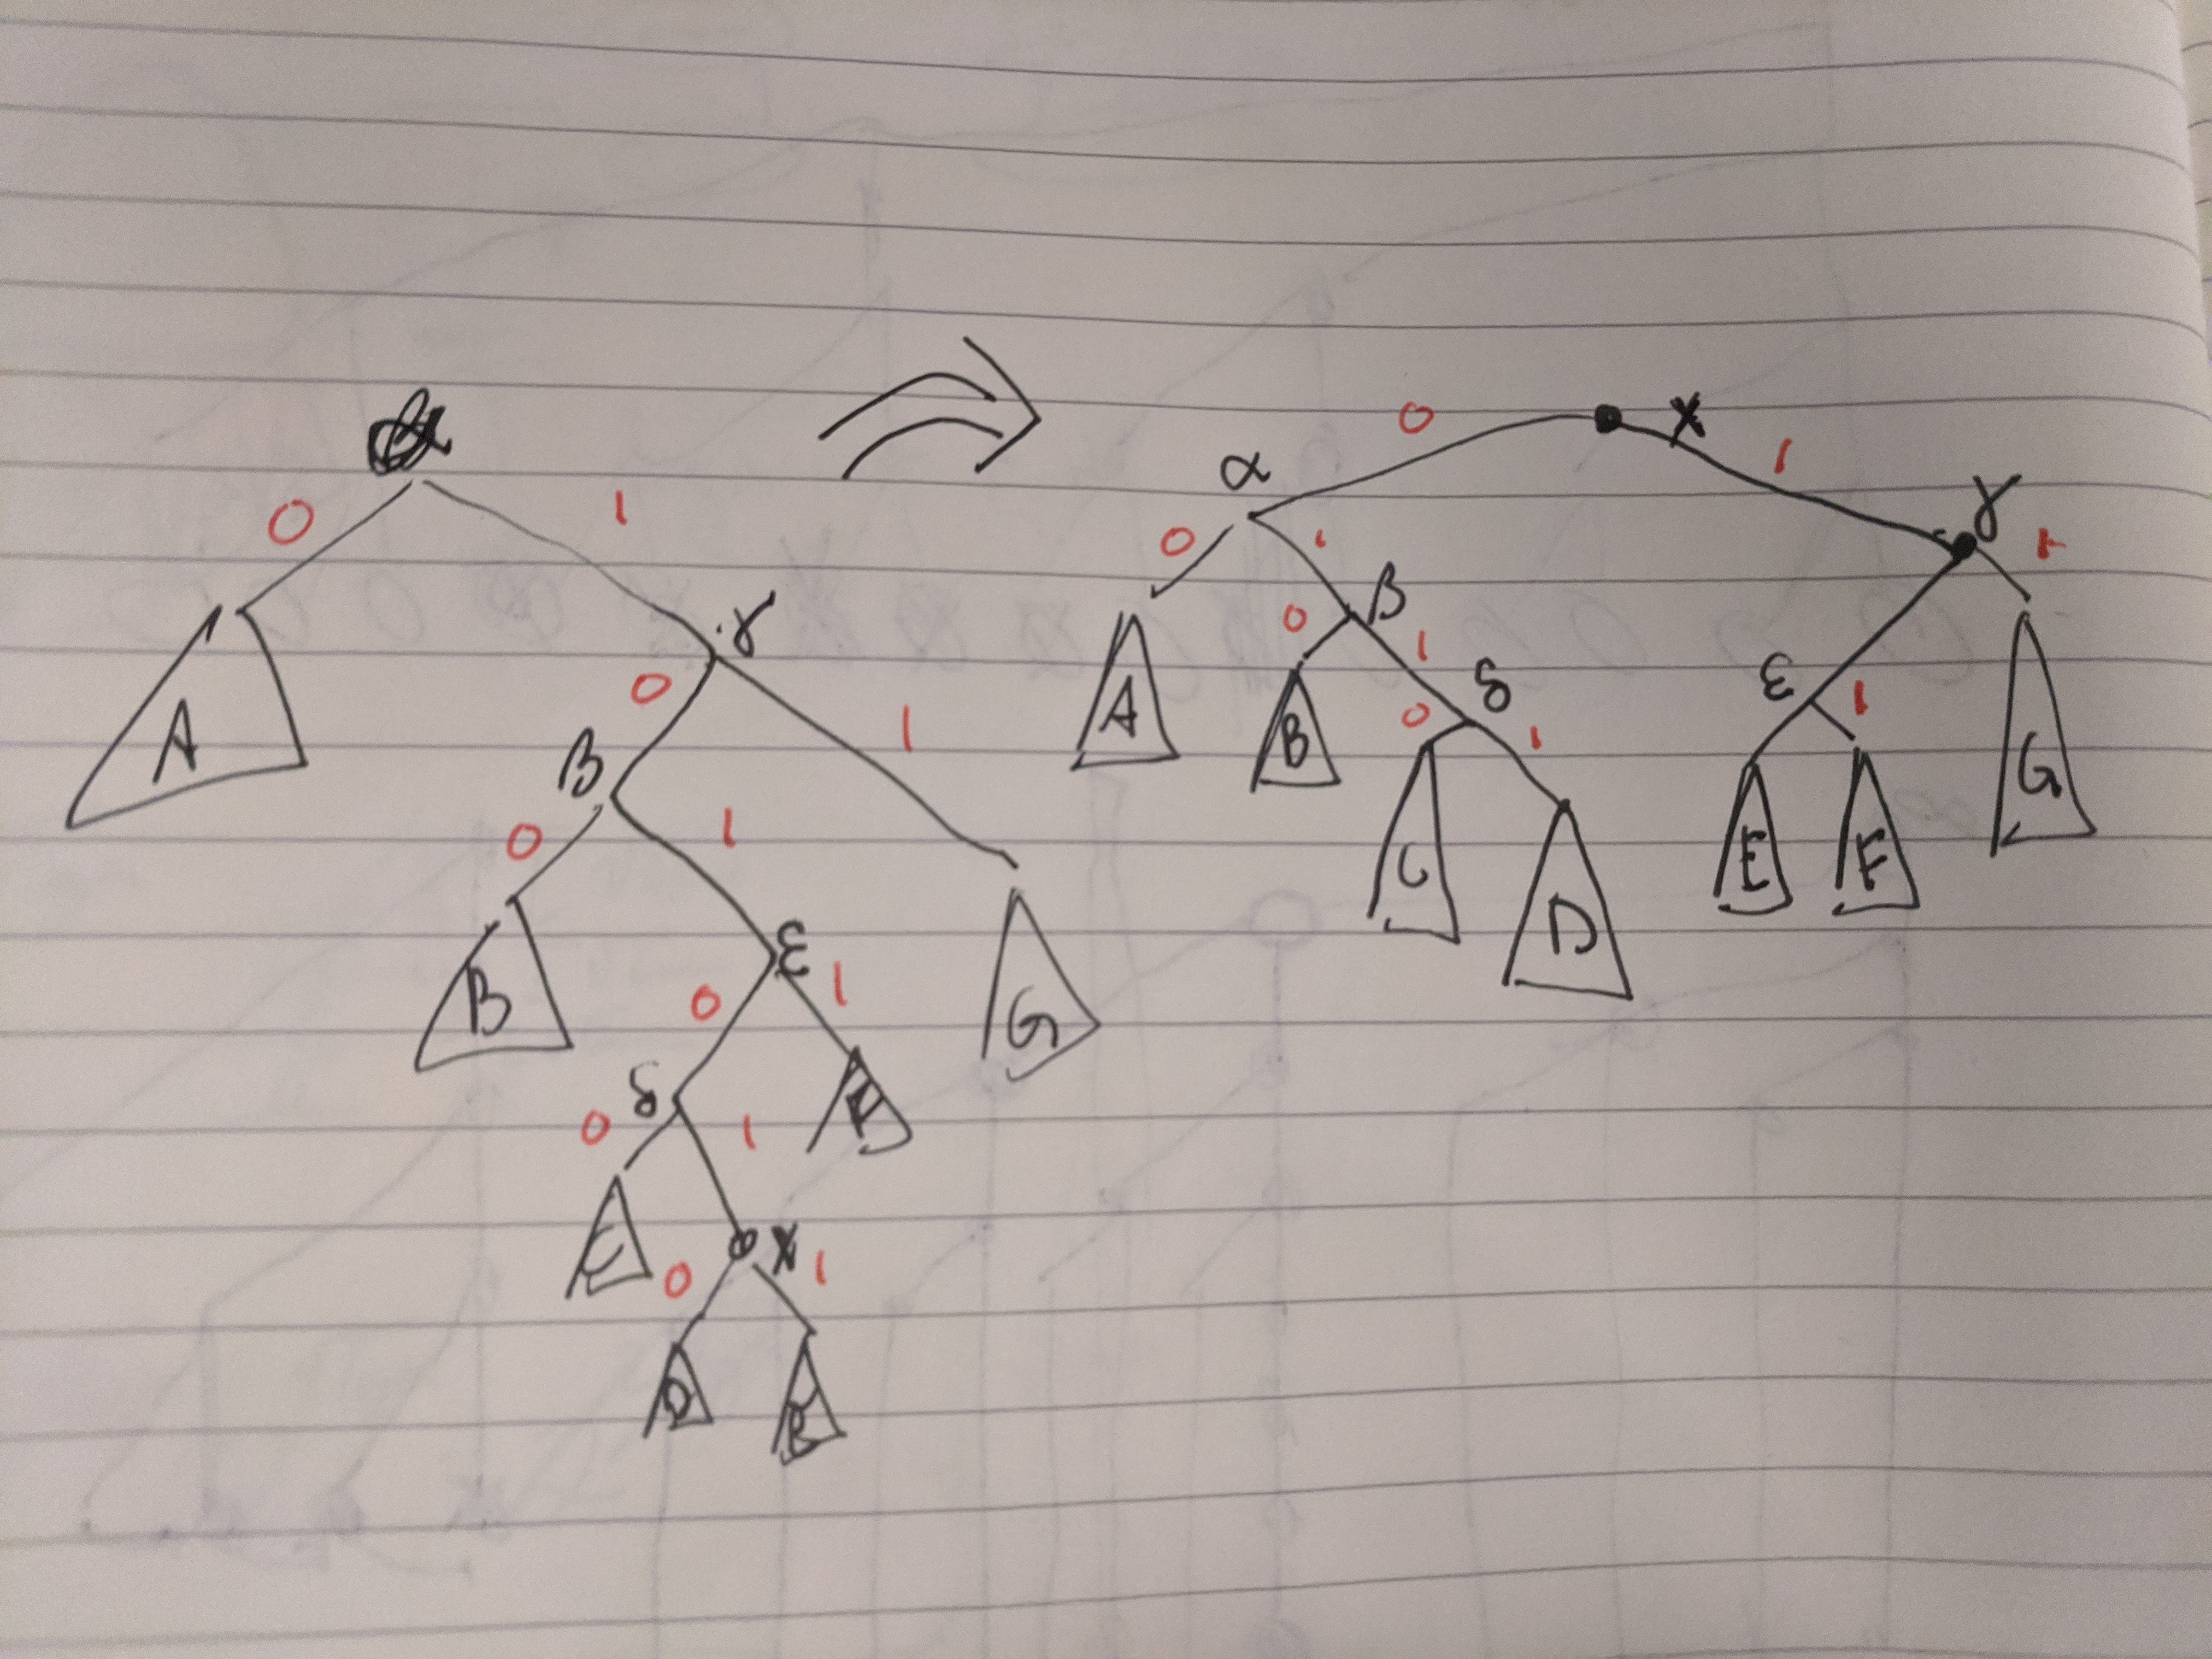
\includegraphics[width=.6\textwidth]{images/split}
  \end{center}
\end{proof}

\lemref{split} allows us to perform a perfect split at the root of $T$ and still maintain an $O(\log h(T))$-length description of the changes required to obtain $\sigma_{T'}(z)$ from $\sigma_T(z)$.  A useful fact about \lemref{split} is that the left and right subtree of $T'$ each have height at most $h(T)$.
The following lemma uses \lemref{split} recursively:

\begin{lem}\lemlabel{mini-split}
  Let $T$ be a binary search tree and let $x_1<\cdots<x_c$ be a set of nodes in $T$. Then there exists a binary search tree $T'$ with $V(T')=V(T)$, $h(T')\le h(T)+\log c$, and in which $T'[\{x_1,\ldots,x_c\}]$ is a tree of height at most $\log c$ that contains the root of $T'$ and such that, for each node $z\in V(T')$, there is a binary string of length $O((1+\log c)\log h(T))$ that describes how to convert $\sigma_T(z)$ into $\sigma_{T'}(z)$.  Furthermore, each tree in the forest $T'-\{x_1,\ldots,x_c\}$ is a tree of height at most $h(T)$.
\end{lem}

\begin{proof}
  The proof is by induction on $c$.  If $c=0$, the statement is trivially true with $T':=T$.  If $c\ge 1$,  apply \lemref{split} to $x_{\lceil c/2\rceil}$ to obtain a tree $T_\times$ rooted at at $x_{\lceil c/2\rceil}$.  Next apply induction on the left subtree of $T_\times$ with the set $x_1,\ldots,x_{\lceil c/2\rceil -1}$ and apply induction on the right subtree of $T_\times$ with the set $x_{\lceil c/2\rceil +1},\ldots,x_c$.  Let $T'$ be the tree whose root is $x_{\lceil c/2\rceil}$ and whose left and right subtrees are the result of these two applications of induction.
  
  It is straitforward to check that $h(T')\le h(T)+\log c)$ and that $T[\{x_1,\ldots,x_c\}]$ is a tree of height at most $\log c$ that contains the root of $T'$.  The condition involving $\sigma_T(z)$ and $\sigma_{T'}(z)$ follows from the fact that any node $z\in V(T)$ is included in a subtree that is involved in at most $\log c$ inductive calls and each such call involves one application of \lemref{split}.  The effect of each application of \lemref{split} on $\sigma_T(z)$ can be recorded by $O(\log h(T))$ bits for a total of $O((1+\log c)\log h(T))$ bits.  Finally, the condition involving the heights of trees in $T'-\{x_1,\ldots,x_c\}$ follows from the fact that the depth of any node $z$ only increases (by 1) for each element of $x_1,\ldots,x_c$ on the path from the root of $T'$ to $y$.
\end{proof}

\begin{lem}\lemlabel{multi-split}
  Let $k,c\ge 1$ be integers, and let $T$ be a binary search tree.  Then there is a binary search tree $T'$ with $V(T')=V(T)$ in which
  \begin{compactenum}
    \item $h(T')\le h(T)+1$; 

    \item  each of the subtrees $T_i'$, $i\in\{1,\ldots,m'\}$ rooted at a depth-$(k+1)$ node of $T'$ has size at most $|T|/2^k$; and
    
    \item for each $x\in V(T)$, there exists an $O(k\log h(T))$-bit description of the changes required to create $\sigma_{T'}(x)$ from $\sigma_T(x)$.
  \end{compactenum}
\end{lem}

\begin{proof}
  Let $Z\subset V(T)$ be the set of at most $2^k-1$ nodes of $T$ of depth less than $k$.  Then $T-Z$ is a forest consisting of $m\le 2^{k}$ trees $T_1,\ldots,T_h$.  Each such tree $T_i$ has height at most $h(T)-k$.
  
  Select the nodes $X:=\{x_1,\ldots,x_{2^k}-1\}$ of $T$ where each $x_j$ has rank $\lfloor j|T|/2^k\rfloor$ in the set $V(T)$.\footnote{For a finite $X\subset\R$, the \emph{rank} of $x\in S$ is $|\{x'\in S: x'<x\}$.}  For each $j\in\{1,\ldots,m\}$, apply \lemref{mini-split} to the subtree $T_j$ with the at most $2^k$ values $Y\cap V(T_j)$ to obtain a new subtree $T_{j}'$.  Let $T^@$ be the tree obtained by replacing each of $T_1,\ldots,T_m$ with $T_1',\ldots,T_m'$, respectively.
  
  Now, $Z\cup X$ has size at most $2(2^{k}-1)< 2^k-1$ and $T^@[Z\cup X]$ is a connected subtree that contains the root of $T^@$.  Construct the tree $T'$ by building a complete binary search tree $T'_0$ of height at most $k$ with $V(T_0')=Z\cup X$ and then attaching each tree in the forest $T^@-(Z\cup X)$ to the appropriate location in $T'_0$.  Since $T'_0$ has height at most $k$ and each tree in this forest has height at most $h(T)-k$, $h(T')\le h(T)+1$.
  
  For the final condition, observe that, for each each node $x\in (Z\cup X)\cap V(T_i)$ we can obtain $\sigma_{T^@}(x)$ from an additional $O(k\log h(T))$ bits as described in \lemref{mini-split}. From $\sigma_{T^@}(x)$ we can obtain $\sigma_{T'}(x)$ by deleting a prefix whose length can be specified using $O(\log h(T))$ bits and replace this with a sequence of at most $k+1$ bits describing a path from the root of $T'_0$ to an external node.\snote{define external node}
\end{proof}

\subsection{Rebalancing}

We can now describe the sequence of binary search trees $T_1,\ldots,T_h$ satisfying (PR1)--(PR4).  Recall that $V(T_i)=V_{i}$ where $V_1,\ldots,V_m$ are the sets described by \lemref{fractional}.  The easiest way to describe these trees is in terms of a binary search tree $T$ that supports two operations:
\begin{enumerate}
  \item \emph{bulk-deletion}: in which a set $D:=V_{i}\setminus V_{i+1}$ of at most $|T|(1-2/a)$ values are removed from $T$. 
  % The set $V_{i+1}=V(T)\setminus D$ of remaining values $a$-chunks $D$.  
  % \pnote{NOTE: We don't use the $a$-chunking property, except for the lower-bound it gives on $|V_{i+1}|$.}
  \item \emph{bulk-insertion}: in which a set $I:=V_{i+1}\setminus V_i$ of at most $2a|T|$ new values are added into $T$.  The set $I$ of newly added values are $a$-chunked by $V(T)$.
\end{enumerate}
First we consider the effect of a pair of bulk-deletion/bulk-insertion operations on the height of $T$.

By \lemref{deletion-prefix}, each bulk-deletion does not increase $h(T)$.  Thus, if we start with a tree $T_1^\times$ and peform one bulk-deletion and one bulk-insertion then, 
by \lemref{chunked-addition}, the resulting tree $T_2$ has height
\[
   h(T_2) \le h(T_1^\times)+1+\log a \enspace .
\]
Thus, a single round of bulk-insertion/bulk-deletion does not increase the height of $T$ by more than $1+\log a$.  The trick is to devise a rebalancing scheme that only allows this to continue for $o(\log n)$ rounds before guaranteeing that the tree returns to a more balanced state.

We will use a rebalancing scheme that is parameterized by an integer parameter $k\in o(\log n)$ to be discussed shortly.  This scheme guarantees that, for each $y\in\{1,\ldots,\lceil\log|T_i|/(k-\log(2a))\rceil+1\}$, 
\begin{enumerate}[(B1)]
  \item $h(T_y)\le h(T_1) + (y-1)(2+\log a)$;
  \item each subtree of $T_y$ rooted at a node of depth $(y-1)(k+1)$ has size at most $|T_1|(2a/2^k)^{y-1}$.
\end{enumerate}

The invariants (B1) and (B2) actually provide two upper bounds on the height of $h(T_y)$.  Let
\[
   y^* := \left\lceil \frac{\log|T_1|}{k-\log(2a)}\right\rceil + 1
\]
and observe that
\[
   |T_{1}|\left(\frac{2a}{2^k}\right)^{y^*-1} \le 1 \enspace .
\]
So, by (B2) every subtree of $T_{y^*}$ of depth $(y^*-1)(k+1)$ has size at most 1.  A subtree of size 1 has height 0.  Therefore,
\begin{align*}
  h(T_{y^*}) & \le (y^*-1)(k+1) \\
  & = \frac{(k+1)\log|T_1|}{k-\log(2a)} + k+1 \\
  & \le \frac{(k+1)(\log |T_{y^*}| + (y^*-1)\log(2a))}{k-\log(2a)} + k+1 \\
  & \le \log|T_{y^*}| + O(k + k^{-1}\log |T_y|) \\
  & \le \log |T_{y^*}| + O(k + k^{-1}\log n)
\end{align*}

Let $r_1=h(T_1)-\log |T_1|$ and note that $|T_y|\ge |T_1|/(2a)^{i-1}$ so, for $i\in\{1,\ldots,i^*\}$, (B1) gives the upper bound
\begin{align}
     h(T_i) & \le h(T_1) + (y-1)(1+\log a) \nonumber \\
            &= \log|T_1| + (y-1)(1+\log a) + r_1 \nonumber \\
            &\le \log |T_y| + (y-1)(1+2\log a) + r_1 \nonumber \\
            &\le \log |T_y| + (y^*-1)(1+2\log a) + r_1 \nonumber \\
            &\le \log |T_y| + O(k^{-1}\log|T_y|) + r_1 \nonumber \\
            &\le \log |T_y| + O(k^{-1}\log n) + r_1 \enspace .
\end{align}

Therefore, if $r_1\in o(\log n)$ and $k\in\omega_{n}(1)$, then
\[  h(T_y) \le \log |T_y| + o(\log n) \]
for all $y\in\{1,\ldots,y^*\}$.  At the end of this process, the tree $T_{y^*}$ has height
\[
    h(T_{y^*})= \log |T_{y^*}| + O(k + (\log n)/k) := \log |T_{y^*}| + r_{y^*}
\]
where $r_{y^*}:=h(T_{y^*})-\log|T_{y^*}|\in O(k + k^{-1}\log n)$.  At this point we continue as if $T_{y^*}$ were the first tree in the sequence.  This is is valid since $r_{y^*}\in o(\log n)$.  This establishes Property~(PR2) for the sequence of trees $T_1,\ldots,T_h$.  

It remains is to describe the rebalancing scheme that guarantees (B1) and (B2).  The scheme is simple: For each $y\in\{1,\ldots,y^*-1\}$,
\begin{enumerate}[(S1)]
  \item Apply \lemref{multi-split} to each of the at most $2^{(y-2)(k+1)}$ subtrees of $T_y$ rooted at nodes of depth $(y-2)(k+1)$ to obtain a new tree $T_y'$.
  \item Perform the bulk-insert operations in $I_y:=V_{y+1}\setminus V_y$ on $T_y'$ to obtain the new tree $T_y''$.
  \item Perform the bulk-delete operations in $D_y:=V_{y}\setminus V_{y+1}$ on $T_y''$ to obtain the new tree $T_{y+1}$.
\end{enumerate}

The proof that these operations preserve invariants (B1) and (B2) is by induction on $y$.  For the base case $y=1$, both properties are trivial: (B1) asserts that $h(T_1)\le h(T_1)$ and (B2) asserts that the subtree of $T_1$ rooted at the root of $T_1$ has size at most $|T_1|$.

For the inductive step, we assume invariants (B1) and (B2) hold for $T_{y-1}$ and prove that they hold for $T_{y}$, $y\ge 2$.  First we establish (B1) as follows:
\begin{align*}  
  h(T_y) & \le h(T_{y-1}'') & \text{(by \lemref{deletion-prefix})} \\
          & \le h(T_{y-1}') + \log a & \text{(by \lemref{chunked-addition})} \\
          & \le h(T_{y-1}) + 1 + \log a & \text{(by \lemref{multi-split})} \\
          & \le h(T_1) + (y-2)(1+\log a) + 1 + \log a & \text{(by (B1) for $T_{y-1}$)}\\
          & = h(T_1) + (y-1)(1+\log a) \enspace ,
\end{align*}
as required.

Next we establish (B2).  By (B2) applied to $T_{y-1}$, every subtree of $T_{y-1}$ rooted at a node of depth $(y-2)(k+1)$ has size at most $|T_{1}|(2a/2^k)^{y-2}$.  Step (S1) then ensures that every subtree of $T_{y-1}'$ rooted at a node of depth $(y-1)(k+1)$ has size at most $|T_{1}|(2a/2^k)^{y-2}/2^k$.  The bulk addition in (S2) increases the size of each subtree by a factor of at most $2a$, so every subtree of $T_{y-1}''$ rooted at a node of depth $(y-1)(k+1)$ has size at most $|T_{1}|(2a/2^k)^{y-1} $.
Finally, the bulk-deletion in (S3) does not increase the size of any subtree, so every subtree of $T_{y}$ rooted at a node of depth $(y-1)(k+1)$ has size at most $|T_{1}|(2a/2^k)^{y-1}$, as required.


\subsection{The $\nu$ Code}

In the previous section we established that the sequence $T_1,\ldots,T_m$ of trees satisfies Property~(PR2) since $|\sigma_{T_y}(x)|\le h(T_y)\le \log |T_y|+O(k+k^{-1}\log n)$.  These trees also satisfy Properties~(PR1) and (PR3) since, for each $y\in\{1,\ldots,h\}$, $V(T_y)=V_y$ is the set described in \lemref{fractional}.  Thus, all that remains is to describe the codes $\nu_y(x)$ for each $y\in\{1,\ldots,h-1\}$ and $x\in V_y\cap V_{y+1}$ that satisfy Property~(PR4).

The purpose of $\nu_y(x)$ is to provide instructions on how to modify $\sigma_{T_y}(x)$ to obtain $\sigma_{T_{y+1}}(x)$.  Therefore we consider the three steps (S1)--(S3) that convert $T_y$ into $T_{y+1}$.  
\begin{enumerate}[(S1)]
  \item applies \lemref{multi-split} to each subtree of $T_y$ at depth $(y-1)(k+1)$ to obtain a new $T_y'$.  Every node $x\in V(T_y)$ is contained in at most one such subtree $T_{y,x}$ that becomes a subtree $T_{y,x}'$ of $T_y'$.  For each such node $x$, we include the integer $(y-1)(k+1)$ in $\nu_y(x)$. \lemref{multi-split} describes $O(k\log h(T))=O(k\log\log n)$ bits that make it possible to recover $\sigma_{T_{y,x}'}(x)$ from $\sigma_{T_{y,x}}(x)$.  To get $\sigma_{T_y'}(x)$ we keep the first $(y-1)(k+1)$ bits of $\sigma_{T_y}(x)$ and append $\sigma_{T_{y,x}'}(x)$.
  
  \item applies \lemref{chunked-addition} (bulk-insertion) to $T_{y}'$ to obtain $T_{y}''$.  This has no effect on any existing signature.  That is, $\sigma_{T_y'}(x)=\sigma_{T_{y}''}(x)$ for every $x\in V(T_i)$.
  
  \item applies \lemref{deletion-prefix} (bulk-deletion) to $T_{y}''$ to obtain $T_{y+1}$. \lemref{deletion-prefix} shows that, for each $x\in V_{y+1}$, $\sigma_{T_{y+1}}(x)$ can be obtained by removing a suffix from $\sigma_{T_y''}(x)$.  For each $x\in V_{y+1}$, the length of this suffix, encoded using $O(\log\log n)$ bits is included in $\nu_{y}(x)$.
\end{enumerate}

This establishes, Property~(PR4) of $T_1,\ldots,T_h$ where each code $\nu_y(x)$ has length at most $O(k\log\log n)$. The optimal choice of $k=\left\lceil\sqrt{\log n/\log\log n}\right\rceil$, which results each vertex of the $n$-vertex subgraph $G$ of $P_1\boxtimes P_2$ being assigned a label of length $\log n + O(\sqrt{\log n\log\log n})$.

\begin{thm}
  There exists an adjacency-labelling scheme for subgraphs of $P_1\boxtimes P_2$ in which the vertices of any $n$-vertex subgraph $G$ of $P\boxtimes P$ are assigned labels of length at most $\log n + O(\sqrt{\log n\log\log n})$.
\end{thm}

\section{Subgraphs of $H\boxtimes P$}

In this section we build on the result of \secref{pxp} to find labelling schemes for graphs $G$ that are subgraphs of $H\boxtimes P$ where $H$ is a $t$-tree and $P=1,2,\ldots,h$ is a path.  Our strategy is similar the approach taken in the previous section.
For each $y\in\{1,\ldots,h\}$ we define $L_y=\{x: (x,y)\in V(G)\}$ and we will build a labelling scheme for the induced graph $H[V_y]$ where $V_y\supseteq L_y$ that is based on a binary tree $T_y$ and such that the labels in this scheme have length $\log|T_y|+o(\log n)$.  In addition to this, we will use \lemref{row-code} so to give each vertex $(x,y)\in V(G)$ a \emph{row label} of length $\log n - \log|T_y|+o(\log n)$.


\subsection{$t$-Trees}

A graph $H$ is a \emph{$t$-tree} if $H$ is a clique on $t$ vertices or if $H$ contains a vertex $v$ of degree $t$ whose neighbours form a clique and $H-v$ is a $t$-tree.  \snote{Use $k$-tree instead?}  

We begin by describing a labelling schemes for $t$-trees. The ideas behind this scheme are not new; this is essentially the labelling scheme for $t$-trees described by Gavoille and Labourel \cite{gavoille.labourel:shorter}.  However, we present these ideas in a manner that makes it natural to generalize the results of \secref{pxp}.

Note that the recursive definition of $t$-trees implies that there is a vertex ordering $v_1,\ldots,v_{m}$ of $V(H)$ such that $v_1,\ldots,v_t$ form a clique and, for each $i\in\{t+1,\ldots,t_m\}$, $C_H(v_i):=B_H(v_i)\cap \{v_1,\ldots,v_{i}\}$ is a clique of size $t+1$.  We call $C_H(v_i)$ the \emph{family clique} of $v_i$ and $C_H(v_i)\setminus\{v_i\}$ the \emph{parent clique} of $v_i$.\snote{TODO: check if we ever use these terms.}  The order $v_1,\ldots,v_m$ is called a \emph{construction order} for $H$.

The order $v_1,\ldots,v_m$ (in particular, the fact that each $v_i$ has at most $t$ neighbours among $v_1,\ldots,v_{i-1}$) implies that $V(H)$ has a proper $(t+1)$-colouring $\varphi:V(H)\to\{1,\ldots,t+1\}$.  For each $i\in\{t+1,\ldots,m\}$ and each $j\in\{1,\ldots,t+1\}$ the \emph{$j$-parent} $p_j(v_i)$ of $v_i$ is the unique element $p\in C_H(v_i)$ with $\varphi(p)=j$.  Note that $v_i$ is the $j$-parent of itself for exactly one $j\in\{1,\ldots,t+1\}$.

\subsection{Interval Graphs}

For real numbers $a\le b$, let $[a,b]:=\{ x\in\R: a\le x\le b\}$, and let
$\mathbb{I}:=\{[a,b]: a,b\in\R,\, a\le b\}$ denote the set of closed real intervals.  For a finite set $S\subset\mathbb{I}$ of intervals, the \emph{interval intersection graph} $G_S$ is the graph with vertex set $V(G_S):=S$ and in which the edge $vw\in E(I)$ if and only if $v\cap w\neq \emptyset$.  

% The \emph{thickness} $\omega(G_S)$ of $S$ is the size of its largest clique, which (by Helly's Theorem) is equal to $\max_{x\in\R}|\{v\in V(H):x\in v\}|$.  By Dilworth's Theorem (applied to the poset $(V(I),\prec)$ where $[a,b]\prec [c,d]$ iff $b<c$), the chromatic number $\chi(I)$ of $I$ is equal to its thickness, i.e., $\chi(I)=\omega(I)$.  

The following well-known result states that every $n$-vertex $t$-tree is the subgraph of an interval graph with thickness $O(t\log n)$:

\begin{lem}\lemlabel{interval-representation}
  For every $n$-vertex $t$-tree $H$, there exists a mapping $f:V(H)\to\mathbb{I}$, such that the interval intersection graph $G_S$ with $S:=\{f(v):v\in V(H)\}$ has thickness at most $\log_{3/2} t\log n$ and, for every $vw\in E(H)$, $f(v)\cap f(w)\neq\emptyset$.  
  
  Furthermore, for every proper $(t+1)$-colouring $\varphi:V(H)\to\{1,\ldots,t+1\}$ of $H$, there exists a proper colouring $\varphi':V(G_S)\to\{1,\ldots,\lceil\log_{3/2} n\rceil\}\times\{1,\ldots,t+1\}$ where, for each $v\in V(H)$, $\varphi'(f(v))=(j,\varphi(v))$ for some $j\in\{1,\ldots,\lceil\log_{3/2} n\rceil\}$.
\end{lem}

In light of \lemref{interval-representation} we will not distinguish between a vertex $v\in V(H)$ and the interval $f(v)$.  That is, we will treat the nodes of every $t$-tree as intervals that satisfy the conditions of \lemref{interval-representation}.

A point $x\in\R$ \emph{stabs} an interval $[a,b]$ if $\{x\}\cap [a,b]=\{x\}$. A finite set $X\subset\R^2$ of points \emph{stabs} a set $S\subset\mathbb{I}$ of intervals if, for every $[a,b]\in S$, at least one point $x\in X$ stabs $[a,b]$, i.e., $X\cap [a,b]\neq\emptyset$.

\snote{TODO: Define ancestor and lowest-common-ancestor}

\begin{lem}\lemlabel{common-ancestor}
  Let $S\subset\mathbb{I}$ be a set of intervals, let $X\subset\R^2$ be a set of points that stabs $S$, and let $T$ be a binary search tree with $V(T):=X$, let $[a,b]\in S$ and let $x$ be the lowest common ancestor, in $T$, of $X\cap [a,b]$.  Then $x\in [a,b]$.
\end{lem}

\begin{proof}
  Since $x$ is the least common ancestor of $X\cap[a,b]$, either $x\in X\cap[a,b]$, in which case there is nothing prove, or there is some pair $x_1,x_2\in X\cap[a,b]$ such that $x_1$ is in the subtree of $T$ rooted at the left child of $x$ and $x_2$ is in the subtree of $T$ rooted at the right child of $x$.  By the binary search tree property, $x_1<x<x_2$. But $x_1,x_2 \in [a,b]$, so $a\le x_1<x<x_2\le b$, so $x\in [a,b]$.  
\end{proof}

\subsection{A Labelling Scheme for $t$-Trees}
\seclabel{t-tree-labelling}

We can use \lemref{common-ancestor} to create a labelling scheme for $t$-trees based on any binary search tree containing stabbing set.  Let $H$ be a $t$-tree whose vertex set $V(H):=S$ consists of the intervals described by \lemref{interval-representation}, let $v_1,\ldots,v_m$ be a construction order for $H$, let $\varphi:V(H)\to\{1,\ldots,t+1\}$ be a proper colouring of $H$, and let $\varphi':V(H)\to\{1,\ldots,\lceil\log_{3/2} n\rceil\}\times\{1,\ldots,t+1\}$ be the extension of $\varphi$ to a proper colouring of $G_S$ described in \lemref{interval-representation}.

Let $X\subset\R$ be any set of points that stab $S$, let $T$ be a binary search tree with $V(T)=X$, and let $\varphi:V(H)\to\{1,2,\ldots,\lfloor t\log n\rfloor\}$ be a proper colouring of the interval graph with vertex set $S$.

For each vertex $v:=[a_v,b_v]\in V(H)$, let $x_T(v)$ denote the lowest-common-ancestor of $X\cap [a_v,b_v]$ in $T$.  For any subset $C\subseteq V(H)$, let $x_T(C):=\{x_T(x):x\in C\}$.  

\begin{lem}\lemlabel{one-path}
  For any $v\in V(H)$ with family clique $C_H(v)$, the set of nodes $x_T(C_H(v))$ are all contained a single root-to-leaf path in $T$.
\end{lem}

\begin{proof}
  Suppose for the sake of contradiction that this is not true, so there are $x_1,x_2\in x_T(C_H(v))$ neither of which is an ancestor of the other.  Then consider the lowest common ancestor $x$ of $x_1$ and $x_2$ in $T$.  Assume without loss of generality that $x_1$ is in the subtree of $T$ rooted at $x$'s left child and $v_2$ is in the subtree of $T$ rooted at $x$'s right child, so $x_1<x<x_2$. The node $x_1:=x_T(v_1)$ for some $v_1:=[a_1,b_1]\in C_H(v)$ and $x_2=x_T(v_2)$ for some $v_2:=[a_2,b_2]\in C_H(v)$.  Since $v_1$ and $v_2$ are both in the family clique $C_H(v)$, the edge $v_1v_2\in E(H)$, and therefore $[a_1,b_1]\cap[a_2,b_2]\neq\emptyset$.  This implies that $x\in [a_i,b_i]$ for at least one $i\in\{1,2\}$.  But this is a contradiction since $x_T(v_i)$ is supposed to be the lowest common ancestor of $[a_i,b_i]\cap X$.
\end{proof}

The following observation shows that a vertex $v$ of $H$ is uniquely identified by $x_T(v)$ and $\varphi'(v)$.

\begin{obs}\obslabel{unique-id}
    For any two distinct vertices $v,w\in V(H)$, $x_T(v)\neq x_T(w)$ or $\varphi'(v)\neq\varphi'(w)$.  Consequently, $\sigma_T(x_T(v))\neq \sigma_T(x_T(w))$ or $\varphi'(v)\neq\varphi'(w)$. 
\end{obs}

\begin{proof}
  If $x_T(v)=x_T(w)=x$, the intervals $v=[a_v,b_v]$ and $w=[a_w,b_w]$ each contain $x$, so $vw\in E(G_S)$.  Therefore $\varphi'(v)\neq\varphi'(w)$ since $\varphi'$ is a proper colouring of $G_S$.  The second, equivalent, statement of the observation is immediate from the fact that the $\sigma_T: V(T)\to\{0,1\}^*$ is injective, so $\sigma_T(x)$ uniquely identifies $x$.
\end{proof}

For each node $v\in V(H)$, let $\sigma_T(v)$ denote the path in $T$ that begins at the root of $T$ and ends at the node in $x_T(C_H(v))$ of maximum depth.  By \lemref{one-path}, $\sigma_T(v)$ contains every node in $x_T(C_H(v))$.
The label for a vertex $v\in V(H)$ consists of the following (we ignore any integers, such as $t$, $|\sigma_T(v)|$, and $\lceil\log_{3/2} m\rceil$, that can be encoded using \lemref{elias}):

\begin{enumerate}[(TC1)]
  \item $\sigma_T(v)$;
  \item $d_T(x_T(p_j(v))$ for each $j\in\{1,\ldots,t+1\}$; 
  \item $\varphi'(p_j(v))$ for each $j\in\{1,\ldots,t+1\}$; and
  \item $\varphi'(v)$.
\end{enumerate}

Given the labels of two vertices $v,w\in V(H)$, we test if $v$ and $w$ are adjacent as follows:
\begin{enumerate}[({A}1)]
  \item If the labels of $v$ and $w$ are identical then $v=w$, so return false.
  
  \item Compute $j:=\varphi(v)$ (which is contained in $\varphi'(v)$), compute $d:=d_T(x_T(p_j(v)))$ and take the length-$d$ prefix of $\sigma_T(v)$ to get $\sigma_T(x_T(v))$.

  \item For each $j\in\{1,\ldots,t+1\}$, compute $d:=d_T(x_T(p_j))$ and take the length-$d$ prefix of $\sigma_T(w)$ to get $\sigma_T(x_T(p_j(w)))$.  If $\sigma_T(x_T(v))=\sigma_T(x_T(p_j(w)))$ and $\varphi'(v)=\varphi'(p_j(w))$ then, by \obsref{unique-id}, $v$ is the $j$-parent of $w$ so $vw\in E(H)$, so return true.
  
  \item[(A4,A5)] Repeat (A2) and (A3) with the roles of $v$ and $w$ reversed.
  
  \item[(A6)] Return false
\end{enumerate}

The correctness of this procedure follows from \obsref{unique-id} (so positive results in (A3) and (A5) are never incorrect) and the fact that, for every $vw\in E(H)$, there exists a $j\in\{1,\ldots,t+1\}$ such that $v$ is the $j$-parent of $w$ or $w$ is the $j$-parent of $v$ (so the negative result in (A6) is never incorrect).  In fact, this labelling scheme proves the slightly stronger result:

\begin{lem}\lemlabel{t-tree-labelling}
  Let $H$, $S$, $X$, and $T$ be defined as above.  There exists a function $\mathds{T}:(\{0,1\}^*)^2\to \Z\cup\{\perp\}$ such that there is a prefix-free code $\gamma:V(H)\to\{0,1\}^*$ where $|\gamma(v)|=h(T) + O(t(\log t + \log h(T)))$ for every $v\in V(H)$ and, for every $v,w\in V(H)$, 
  \[
      \mathds{T}(\gamma(v),\gamma(w)) = \begin{cases}
      0 & \text{if $v=w$} \\
      -j & \text{if $v$ is the $j$-parent of $w$} \\
      j & \text{if $w$ is the $j$-parent of $v$} \\
      \perp & \text{otherwise.}
    \end{cases}
  \]
\end{lem}

\begin{proof}
  Most of the details of this labelling are described above, though we have thus far ignored the length of the labels, which we analyze now.
  
  Part (TC1) of each label has length $|\sigma_T(v)|\le h(T)$.  For each $x\in V(T)$, $d_T(x)\le h(T)$, so Part~(TC2) of each label requires $O(t\log h(T))$ bits.  Part~(TC3) of each label requires $O(t\log t + t\log h(T))$ bits.  Part~(TC4) of each label requires $O(\log t + \log h(T))$ bits.
\end{proof}

Taking $X$ to be a minimal set that stabs $S$ (so $|X|\le |S|=m$) and taking $T$ to be a perfectly balanced binary search tree (so $h(T)\le \log|X|\le\log m$) we obtain the following corollary.

\begin{cor}\corlabel{t-tree-labelling}
  There exists a function $\mathds{T}:(\{0,1\}^*)^2\to \Z\cup\{\perp\}$ such that, for any $m$-vertex $t$-tree $H$ there is a prefix-free code $\gamma:V(H)\to\{0,1\}^*$ where $|\gamma(v)|=\log m + O(t(\log t + \log\log m))$ for every $v\in V(H)$ and, for every $v,w\in V(H)$, 
  \[
      \mathds{T}(\gamma(v),\gamma(w)) = \begin{cases}
      0 & \text{if $v=w$} \\
      -j & \text{if $v$ is the $j$-parent of $w$} \\
      j & \text{if $w$ is the $j$-parent of $v$} \\
      \perp & \text{otherwise.}
    \end{cases}
  \]
\end{cor}


\subsection{Data Structuring and the $\mu$ Code}

We point out again that the result in \corref{t-tree-labelling} is not new and the labelling scheme is just a reformulation of the one given by Gavoille and Labourel \cite{gavoille.labourel:shorter} that happens to be convenient for what we are going to do next. Most important for us is that the largest part of the codes come from paths in the binary search tree $T$ that contains the stabbing set $X$.  

What we will do next is to show that the solution presented in \secref{pxp} generalizes to the current setting.  The only additional complication comes from the fact that each node $x$ in the binary search tree $T$ is equipped with a collection $B_x:=\{v\in V(H):x_T(v)=x\}$ of intervals.  Any structural changes that we make to $T$ may result in changes to $B_x$, which result in changes to the labels for the vertices of $H$ that enter or leave $B_x$.  We must show that these changes can be encoded using few bits.  We now proceed.

Let $G$ be an $n$-vertex subgraph of $H\boxtimes P$ where $H$ is a $t$-tree and $P=1,\ldots,h$ is a path. For each $y\in\{1,\ldots,h\}$, let $S_y=\{v\in V(H): (v,y)\in V(G)\}$ \snote{Consistency: $S_y$ was $L_y$ in \secref{pxp}} and let $S^-_y=\bigcup_{j=1}^{t+1}\{p_j(v):v\in S_y\}$.  Note that $|S^-_y|\le t|S_y|$. For each $y\in\{1,\ldots,t+1\}$, let $X_y\subset\R$ be the set of all endpoints of intervals in $S^-_y$.  Note that $|X_y|$ stabs $S^-_y$.

Now apply the result of \secref{pxp} to get a sequence of trees $T_1,\ldots,T_h$ where, for each $y\in\{1,\ldots,m\}$, 
\begin{enumerate}[(PRX1)]
  \item $V(T_y)\supseteq X_y$;
  \item $h(T_y)\in \log |T_y| + o(\log n)$;
  \item $W:=\sum_{y=1}^h |T_y|\in O(n)$; and
  \item There is a function $B:(\{0,1\}^*)^2\to\{0,1\}^*$ such that, for every $x\in V(T_y)\cap V(T_{y+1})$, there is an $o(\log n)$-bit string $\nu_y(x)$ such that $B(\sigma_{T_y}(x),\nu_y(x))=\sigma_{T_{y+1}(x)}$.
\end{enumerate}

As before, we can use \lemref{row-code} to assign each vertex $v=(x,y)\in V(G)$ a label $\alpha(v)$ of length $\log n - \log|T_y| + o(\log n)$. For any two nodes $v_1=(x_1,y_1)\in V(G)$ and $v_2=(x_2,y_2)$, $\alpha(v_1)$ and $\alpha(v_2)$ are sufficient to determine if $|y_1-y_2|\le 1$ and, if so, the actual value of $y_1-y_2$.

Now, for each $y\in\{1,\ldots,h\}$, $V(T_y)$ stabs $S^-_y$, so we can use $T_y$ to create a labelling scheme $\gamma_y:S^-_y\to\{0,1\}^*$ for the induced graph $H[S^-_y]$ as described in \secref{t-tree-labelling} leading to \lemref{t-tree-labelling} where the labels have length $h(T_y) + o(\log n)=\log|T_y|+o(\log n)$.  

For each $v\in S^-_y$, the label $\gamma_y(v)$ has four parts (TC1)--(TC4).  Parts~(TC3) and (TC4) are completely determined by $H$ and $v$ and are independent of $T_y$.  In particular parts (TC3) and (TC4) of $\gamma_{y_1}(v)$ and $\gamma_{y_2}(v)$ are the same for any $y_1$ and $y_2$ such that $(v,y_1),(v,y_2)\in V(G)$.  

Part~(TC2) of $\gamma_y(v)$, however depends very much on the tree $T_y$.  Luckily, Part~(TC2) is small: It has size $o(\log n)$, so the label of $(v,y)$ can include Part~(TC2) for $\gamma_{y}(v)$ and $\gamma_{y+1}(v)$.\snote{Do we need $\gamma_{y-1}(v)$ also?}

The difficulty comes from Part~(TC1) of $\gamma_y(v)$.  This part, $\sigma_{T_y}(v)$, is determined by the path from the root of $T_y$ to the deepest node $z\in x_{T_y}(C_H(v))$.  When $T_y$ is restructured to become $T_{y+1}$, the path defining $\sigma_{T_y}(v)$ changes, the relative depths of nodes in $x_{T_y}(C_H(v))$ may change and even the value $x_{T_y}(w)$ may change for any $w\in V(H)$.  

We now examine the three operations that define how $T_y$ is transformed into $T_{y+1}$ to show how the effects of these operations on the labels of nodes in $S^-_y\cap S^-_{y+1}$ can be encoded succinctly.  Recall that these three operations are (S1)~rebalancing, (S2)~bulk insertion and (S3)~bulk deletion.  
Rebalancing takes $T_y$ onto a tree $T_y'$. Bulk insertion takes $T_y'$ onto a tree $T_y''$.  Bulk deletion takes $T_y''$ onto $T_{y+1}$.


\paragraph{(S1): Rebalancing}

The rebalancing operation involves applying \lemref{multi-split} to all the subtrees of $T$ rooted at nodes of depth $(i-1)(k+1)$.  This, in turn, involves applying \lemref{split} to $2^k-1$ nodes so that they become roots of specific subtrees.

For a binary tree $T$ and a node $z\in V(T)$, let $P_T(z)$ denote the path from the root of $T$ to $z$.  We begin with a simple observation about the restructing operation in \lemref{split}.

\begin{obs}\obslabel{x-switch}
  Let $T$ be a binary search tree and $S$ be a set of intervals and let $T'$ be the result of applying \lemref{split} to $T$ to make node $x'$ become the root.  Then, for each $v=[a,b]\in S$, if $x_{T'}(v)\in\{x_T(v), x\}$.
\end{obs}

\begin{proof}
  Consider any node $z\in V(T)$ and without loss of generality, assume $z>x'$. 
  If $x'$ is not in the subtree of $T$ rooted at $z$, then $P_T(z)=P_{T'}(z)$.  If $x'$ is in the subtree of $T$ rooted at $z$, then $P_T(z)$ is obtained by deleting all values less than $x'$ from $P_T(z)$ and (possibly) inserting $x'$.
  
  Now, consider any $v=[a,b]\in S$ and let $x:=x_T(v)$. By definition, $x$ is is the only node in $P_T(x)$ contained in $[a,b]$. Therefore, the only nodes of $P_{T'}(x)$ contained in $[a,b]$ are $x$ and (possibly) $x'$.  Therefore $x_{T'}(v)\in \{x,x'\}$.
\end{proof}

For any $v\in S^-_{y}\cap S^-_{y+1}$, and any $y\in\{1,\ldots,h\}$, let $P_{T_y}(v)=x_0,\ldots,x_r$ be the path from the root of $T_y$ to the deepest node in $x_{T_y}(C_H(v))$.  In other words, $\sigma_{T_y}(v)=\sigma_{T_y}(x_r)$ and $x_r=x_{T_y}(w)$ for some $w\in C_H(v)$.

A rebalancing operation applies \lemref{multi-split} to each subtree of $T_y$ rooted at a node of depth $(i-1)(k+1)$.  At most one of these subtrees contains nodes from $P_{T_y}(v)$. We first establish that none of the other application of \lemref{multi-split} has any effect on $\sigma_{T_y}(v)$.  Let $T_y^0$ be the result of applying \lemref{multi-split} to every subtree rooted at a depth $(i-1)(k+1)$ node that does not contain any nodes of $P_{T_y}(v)$.
By \obsref{x-switch}, $x_{T_y}(u)=x_{T_y^0}(u)$ for all $u\in C_H(v)$.  The path $P_{T_y}(v)=x_0,\ldots,x_r$ is also a path in $T_y^0$ and this is the path in $T_y^0$ from the root to the deepest node in $x_{T_y^0}(C_H(v))$. So, by definition, $P_{T_y}(v)=P_{T_y^0}(v)$.

Let $T_y'$ be the result of applying \lemref{multi-split} to the subtree $T_*$ of $T_y^0$ that contains some nodes of $P_{T_y}(v)=P_{T_y^0}(v)=x_0,\ldots,x_r$ and let $T_*'$ denote the result of applying \lemref{multi-split} to $T_*$.
The subtree $T_*$ contains some suffix $x_i,\ldots,x_r$ of $x_0,\ldots,x_r$.  By definition $x_r=x_{T_y}(w)$ for some $w=[a_w,b_w]\in C_H(v)$.  Since the only restructuring done by \lemref{multi-split} is done by applications of \lemref{split} to subtrees contained in $T_*$,  \obsref{x-switch} implies that $x_{T_y'}(w)\in V(T_*)$.  Therefore $P_{T_y'}=x_0,\ldots,x_{i-1},x'_0,\ldots,x'_{s}$ where $x_0',\ldots,x'_s$ is a path in $T_*'$. By including the integer $(i-1)(k+1)$ in the label for $(v,y)$, we can therefore focus on encoding the differences between $\sigma_{T_*}(x_r)$ and $\sigma_{T_*'}(x'_s)$.

To simplify notation, we now assume that $T^*=T_y$, so that the one application of \lemref{multi-split} that affects $P_{T_y}(v)$ is at the root of $T_y$.
This application of \lemref{multi-split} involves several applications of \lemref{split}.  Consider the first application of \lemref{split}, that takes some node $x'$ in $T_y$ and moves it to the root, creating a new tree $T_y^1$.

By \obsref{x-switch} $x_{T_y^1}(w)\in\{x',x_{T_y^1}(w)$ for every $w\in C_H(v)$.  If $x_{T_y^1}(w)=x'$ for every $w\in C_H(v)$, then $P_{T_y^1}(v)=x'$ is a path of length 0.  This can be recorded by adding $O(1)$ bits to the label of $(v,y)$. Otherwise, there is a non-empty subset $W\subset C_H(v)$ such that $x_{T_y^1}(w)=x_{T_y}(w)$ for each $w\in W$.  Let $w^*\in W$ be an element that maximizes $d_{T_y}(w^*)$.  We claim that $w^*$ also maximizes $d_{T_y^1}(w^*)$.  Indeed, as noted already in the proof of \obsref{x-switch} $P_{T_y^1}(w^*)$ consists of $x'$ followed by a subsequence of $P_{T_y}(w^*)$ that includes every node in $W$.

Therefore $P_{T_y^1}(v)=P_{T_y^1}(w^*)$.  Now $w^*$ appear in $P_{T_y}(v)$, so $\sigma_{T_y}(w^*)$ can be recovered from $\sigma_{T_y}(v)$ and $d_{T_y}(w^*)$, so the $O(\log\log n)$ bits required to encode $d_{T_y}(w^*)$ are included in the label of $(v,y)$.  Furthermore, as shown in \lemref{split}, $\sigma_{T_y^1}(w^*)=\sigma_{T_y^1}(v)$ can be recovered from $\sigma_{T_y}(w^*)$ and an additional $O(\log\log n)$ bits that are included in the label of $(v,y)$.  In this way, we can recover $\sigma_{T_y^1}(v)$ with the addition of only $O(\log\log n)$ bits to the label of $(v,y)$.

Now \lemref{multi-split} involves $2^k-1$ applications of \lemref{split} resulting in intermediate trees $T_y^1,\ldots,T_y^{2^k-1}=T_y'$.  However, these applications are partitioned into $k$ sets $S_0,\ldots,S_{k-1}$, where the applications of \lemref{multi-split} in $S_i$ operate on $2^i$ disjoint subtrees rooted at nodes of depth $i$.  In particular, only one subtree in each set contains any nodes from $P_{T}(v)$.  Each of these applications adds $O(\log\log n)$ bits to the label of $(v,y)$ for a total of $O(k\log\log n)$ bits.

With these additional bits, we can recover $\sigma_{T_y'}(v)$ from $\sigma_{T_y}(v)$ for every $v\in S^-_y\cap S^-_{y+1}$.

\paragraph{(S2): Bulk-Insertions}

During the bulk-insertion phase, elements in $I_y:=X_{y+1}\setminus X_y$ are added to $T_y'$ to create the new tree $T_{y}''$.  The newly added elements are added to small complete binary search trees that are attached to existing nodes of $T_{y}'$.  This ensures that, in $T_y''$, no vertex of $T_y$ has any ancestor in $I_y$.  This in turn ensures that $x_{T_y''}(v)=x_{T_y'}(v)$ for every $v\in S_y$.  This ensures that $P_{T''}(v)=P_{T'}(v)$, so $\sigma_{T''}(v)=\sigma_{T'}(v)$ for every $v\in S_y$.

\paragraph{(S3): Bulk-Deletions}

Each individual deletion either involves removing a leaf from $T_y''$ or it involves (possibly repeatedly) replacing some value $x$ with some value $x'$ that either the smallest value in $x$'s right subtree or the largest value in $x$'s left subtree.

Let $v=[a_v,b_v]$ be any vertex such that $(v,y)$ and $(v,y+1)$ are both present in $G$.  Recall that, by definition, $a_v$ and $b_v$ are both contained in $X_y$ and in $X_{y+1}$.  If $x_{T_y''}(v)=x$, then $x\in[a_v,b_v]$ and, since $a_v,b_v\in X_{y}$, $x'\in[a_v,b_v]$.  Therefore, if $x_{T''}(v)=x$ then, after replacing $x$ with $x'$, $x_{T''}(v)=x'$.  

The only other possible change of this type occurs when this replacement operation causes $x'$ to become an ancestor of some node $x''$ that it wasn't before.  In this case, some $v\in S_y$ with $x_{T_y''}(v)=x''$ before the replacement will have $x_{T_y''}(v)=x'$ after the replacement.

In either of the preceding cases replacing $x$ with $x'$ has the effect of removing a (possibly empty) suffix from $\sigma_T(x_{T_y}(v))$ for each $v\in S_y$.  Therefore, any number of these operations can only make $\sigma_{T_y}(v)$ shorter.  Therefore, the effect of all these operations on $\sigma_T(v)$ can be represented by one integer $d\in \{0,\ldots,h(T_y'')\}$ that can be represented using $O(\log\log n)$ bits.   We can therefore recover $\sigma_{T_{y+1}}(v)$ by deleting a suffix of length $d$ from $\sigma_{T_y''}(v)$.

In summary, for each $v\in S_y$, there is a bitstring $\mu_y(v)$ of length $O(k\log\log n)$ that allows us to compute $\sigma_{T_{y+1}}(v)$ from $\sigma_{T_y}(v)$.


\subsection{Adjacency Testing}

Summarizing, we have a labelling scheme for any $n$-vertex subgraph $G$ of $H\boxtimes P$ that contains the following information for each vertex $z=(v,y)\in V(G)$:

\begin{enumerate}[(PC1)]
  \item $\alpha(y)$; % of length $\log n-\log|T_y| + O(\log\log n)$;
  \item $\sigma_{T_y}(v)$; % of length $\log|T_y| + O(k+k^{-1}\log n)$;
  \item $d_{T_{y+b}}(x_{T_{y+b}}(p_j(v))$ for each $j\in\{1,\ldots,t+1\}$ and $b\in\{-1,0,1\}$; 
  \item $\varphi'(p_j(v))$ for each $j\in\{1,\ldots,t+1\}$;
  \item $\varphi'(v)$;
  \item $\mu_y(v)$;
  \item $a(z)$.
\end{enumerate}
The only one of these quantities not yet defined is $a(z)$, which is a sequence of $3t$ bits that indicate which of the potential edges joining $z$ to elements of $\{(p_j(v),y+b): j\in\{1,\ldots,t+1\},\, b\in\{-1,0,1\}\}$ are actually present in $G$.

Given the labels of $z_1:=(v_1,y_1)$ and $z_2:=(v_2,y_2)$ we test if $z_1z_2\in E(G)$ by first using $\alpha(y_1)$ and $\alpha(y_2)$ to determine which of the following applies:
\begin{enumerate}
  \item $|y_1-y_2|>1$: In this case $y_1\neq y_2$ and $y_1y_2\not\in P$, so $z_1z_2\not\in E(H\boxtimes P)$, so $z_1z_2\not\in E(G)$.

  \item $y_1=y_2$.  Let $y=y_1=y_2$.  In this case (PC2)--(PC4) contains $\gamma_{H_y}(v_1)$ and $\gamma_{H_y}(v_2)$ and we use this to test if $v_1v_2\in E(H)$.  If not, then $v_1v_2\not\in E(H\boxtimes P)$ so $z_1z_2\not\in E(G)$.  
  
  If $v_1v_2\in E(H)$ then we know that $z_1z_2\in E(H\boxtimes P)$.  In this case $\gamma_{H_y}(v_1)$ and $\gamma_{H_y}(v_2)$ also tell us that (without loss of generality) $x_1$ is the $j$-parent of $x_2$.  We can now consult the relevant bit of $a(z_1)$ to determine if $z_1z_2\in E(G)$.

  \item $y_2-y_1=1$: Let $y=y_1$ (so that $y_2=y+1$).  We use $\mu_y(v_1)$ and $\sigma_{T_y}(v_1)$ to compute $\sigma_{T_{y+1}}(v_1)$.  Now, $\sigma_{T_{y+1}}(v_1)$ and (PC3)--(PC4) contains $\gamma_{H_{y+1}}(v_1)$ and (PC2)--(PC4) contains $\gamma_{H_{y+1}}(v_2)$.  We use these to test if $v_1v_2\in E(H)$.  If not, then $v_1v_2\not\in E(H\boxtimes P)$ so $z_1z_2\not\in E(G)$.  
  
  If $v_1v_2\in E(H)$ then we know that $z_1z_2\in E(H\boxtimes P)$.  In this case $\gamma_{H_{y+1}}(v_1)$ and $\gamma_{H_{y+1}}(v_2)$ also tell us that (without loss of generality) $v_1$ is the $j$-parent of $v_2$.  We can now consult the relevant bit of $a(z_1)$ to determine if $z_1z_2\in E(G)$.

  \item $y_2-y_1=-1$:  This case is symmetric to the preceding case, with the roles of $z_1$ and $z_2$ reversed.
\end{enumerate}

This completes the proof of our main result.

\begin{thm}
  There exists a function $\mathds{A}:(\{0,1\}^*)^2\to\{0,1\}$ such that for every $t$-tree $H$, every path $P$, and every $n$-vertex subgraph $G$ of $H\boxtimes P$, there is a prefix-free code $\eta:V(G)\to\{0,1\}^*$ such that
  $|\eta(v)|=\log n + O(\sqrt{\log n\log\log n}+t(\log t + \log\log n))$ for every $v\in V(G)$ and, for every $v,w\in V(G)$, 
  \[  \mathds{A}(\eta(v),\eta(w)) = \begin{cases}
        1 & \text{if $vw\in E(G)$} \\
        0 & \text{if $vw\not\in E(G)$}
      \end{cases}
      \]
\end{thm}

\section{Conclusion}


\section*{Acknowledgement}

Part of this research was conducted during the Eighth Workshop on Geometry and Graphs, held at the Bellairs Research Institute, January~31--February~7, 2020.  We are grateful to the organizers and participants for providing a stimulating research environment.


% 
% the value $x'$ must be 
% 
% 
% 
% Furthermore, the labels defined by $\gamma$
% 
% The label of each vertex $v=(x,y)\in V(H)$ also includes an array $a$ of $3(t+1)$ bits that indicate whether $G$ contains the edges from $v$ to $w$ for each $w\in\{(p_j(x),y+b):j\in\{1,\ldots,t+1\},\, b=\{-1,0,1\}\}$. 
% 
% The label of each vertex $v=(x,y)\in V(H)$
% 
% 
% 
% We have not yet completed the description of our labelling scheme. Nevertheless, this is a good time to see what information we are still missing.
% At this point, if we are given the labels of two vertices $v_1=(x_1,y_1)$ and $v_2=(x_2,y_2)$ in $V(G)$. We can use $\alpha(v_1)$ and $\alpha(v_2)$ to determine which of the following applies:
% \begin{enumerate}
%   \item $|y_1-y_2|>1$: In this case $y_1\neq y_2$ and $y_1y_2\not\in P$, so $v_1v_2\not\in E(H\boxtimes P)$, so $vw\not\in E(G)$.
% 
%   \item $y_1=y_2$.  In this case we can use $\gamma(v_1)$ and $\gamma(v_2)$ to check if $x_1x_2\in E(H)$.  If not, then $v_1v_2\not\in E(H\boxtimes P)$ so $vw\not\in E(G)$.  If $x_1x_2\in E(H)$ then we know that $vw\in E(H\boxtimes P)$.  In this case $\gamma(v_1)$ and $\gamma(v_2)$ also tell us that (without loss of generality) $x_1$ is the $j$-parent of $x_2$.  We can now consult the relevant bit of $a(x_2)$ to determine if $x_1x_2\in E(G)$.
% 
%   \item $y_1-y_2=1$: Let $y=y_1$ (so that $y_2=y-1$).  In this case $\nu_{y-1}(x_{T_{y-1}}(x_2))$ and $\sigma_{T_{y-1}}(x_2)$ are sufficient to determine $\sigma_{T_{y}}(x_2)$.     \snote{Ack: annoying name conflict $x_T(v)$ and $x\in V(H)$.}
% \end{enumerate}
% 
% 
% 
% 
% 
% 
% 
% 
% 
% 
% 
% 
% 
% 
% 
% 
% 
% 
% 
% 
% 
% 
% 
% 
% 
% 
% 
% \newpage
% 
% 
% \begin{verbatim}
% Hi All,
% 
% Today's progress report:
% 
% 1. I spent time carefully writing the P*P solution---in particular
% finishing up the bulk-insertions/deletions and rebalancing parts.  We
% get label length log n + O(sqrt(log n loglog n).
% http://cglab.ca/~morin/publications/drafts/labelling/
% 
% 2. Vida and I spent some time thinking about the generalization to H*P
% where H is a k-tree, and think that most of the work is done already
% by the P*P solution.  Here's the idea:
% 
% H is a subgraph of an interval graph of thickness k*log n, so let's
% assume the nodes of H are actually real intervals that are properly
% coloured with klog n colours.
% 
% For any subset S of V(H) there is a set X of at most |S| real numbers
% (I'll call these points) so that every v in S contains at least one
% point in X.  We say that X stabs S.
% 
% Our subgraph of H*P actually contains a sequence S_1,..,S_m of subsets
% of V(H) of total size n.  We can greedily compute a sequence of point
% sets  X_1,...,X_m where X_i stabs S_i and there is a function f_i:S_i->x_i
% such that f_i(v) is a point that stabs v.  These point sets are
% constructed lazily so that, if v is in S_i\cap S_{i+1}, then f_i(v)=f_{i+1}(v). 
% The only points in X_i that are not in X_{i+1} are those that are unnecessary: those x in X_i such that there is no v in S_i with f(v)=x.
% 
% This guarantees that |X_i|<=|S_i|.
% 
% Now we're going to use all the machinery we developed in Section 3 of
% the write-up to make a sequence of binary search trees T_1,..,T_m
% where each T_i contains a superset of X_i, the T_i's have linear total
% size, the height of T_i is log|T_i| + o(log n) and, for any point x
% that appears in T_i and T_{i+1}, there is a o(log n)-bit description
% of how to rewrite the root to x path in T_i (a sequence of 0's and
% 1's) so that it becomes the root to x path in T_{i+1}.
% 
% We can also assign a label to each vertex v in S_i of length log n -
% log|T_i| so that for v in S_i and w in S_j, label(v) and label(w) tell
% us if j-i is {-1, 0, 1, >=2}. So now each vertex v in S_i has log|T_i|
% free bits it can still use for its label.
% 
% For each interval/vertex v in S_i, we assign v to the highest point 
% x_i(v) in T_i that stabs v.  Now for any v in S_i, there is one 
% root to leaf path in T_i that contains x(v),x(p_1(v)),..,x(p_k'(v)) where
% p_1(v),..,p_k'(v) are the k-tree parents of v that happen to be in
% S_i.  So log|T_i| + o(log n) bits plus an additional kloglog n bits is
% enough then to recover all the root to x(v) and x(p_i) paths. This
% plus a bit more bookkeeping that Cyril described in his email is
% enough to test if an edge vw is in E(G) using label(v) and label(w)
% provided that v and w are both in S_i.  The only issue that remains is
% what to do if v is in S_i and w is in S_{i+1}, since label(v) contains
% a path to x_i(v) in T_i and label(w) contains a path to x_{i+1}(v) in
% T_{i+1}.  If x_i(v)=x_{i+1}(v) then we're happy: Our solution for P*P
% already includes enough information to convert the path to x(v) in T_i
% into the path to x(v) in T_{i+1}.
% 
% What to do when x_i(v)!= x_{i+1}(v)?  For this, we have to look at why
% x_i(v) would change.  This happens because in T_i, x_i(v) was closer
% to the root than x_{i+1}(v) but in T_{i+1}, x_{i+1}(v) is closer to
% the root than x_i.   How did x_{i+1}(v) get closer to the root in
% T_{i+1}?  For that, we have to look at the solution for P*P and how
% the binary search trees T_i and T_{i+1} are related.
% 
% 1. It wasn't because x_{i+1}(v) was inserted in T_{i+1}: Newly
% inserted nodes are added as tiny subtrees at the leaves. They're
% further from the root than any preexisting node.
% 
% 2. Maybe it was because some ancestor x of x_{i+1}(v) was deleted so
% x_{i+1}(v) took its place, closer to the root.  If so, then the path
% to x_{i+1}(v) in T_{i+1}(v) is still a prefix of path to x_i(v) in
% T_i, and all we need is to store the length of this prefix so we can
% derive the path the root to x_{i+1}(v) path from x_i(v).
% 
% 3. Maybe it was because we did a rebalancing operation that brought
% x_{i+1}(v) closer to the root, overtaking x_i(v).  These rebalancing
% operations all use the same basic operation, and this operation is
% depicted in the only figure in the paper, which I will now refer to.
% In this case, the only nodes on a root-to-leaf path that change
% relative order are on the path to the node x that is being moved
% closer to the root.  Even then, the relative distance to the root of
% these nodes does not change except for nodes a and b where a is on the
% "left wall" of the figure and b is on the "right wall".  But if a
% stabs v and b stabs v, then the root also stabs v.  So the node
% x_{i+1}(v) is the root x in T_{i+1} of subtree being restructured. In
% particular, the root to x path in T_{i+1} is a prefix of the root to
% x_i(v) path in T_i.  This can also be recorded using O(\log\log n)
% bits.
% 
% That's it(?!)
% 
% Pat
% \end{verbatim}
  
  
\bibliographystyle{plainurl}
\bibliography{labelling}

\end{document}
